\chapter*{Referenced Books}
\addcontentsline{toc}{chapter}{Referenced Books}

These cover snapshots identify the editions of the books referenced in this
volume. They are reproduced at small size for bibliographic identification.

\begin{center}
\begin{minipage}[t]{.46\textwidth}
  \centering
  
\includegraphics[height=1.9in,keepaspectratio]{assets/logic-language-models-cover.jpg}\par
  \smallskip
  \small\emph{Logic and Language Models for Computer Science}\par
  Dana Richards and Henry Hamburger \citep{richards2017logic}
\end{minipage}
\hfill
\begin{minipage}[t]{.46\textwidth}
  \centering
  
\includegraphics[height=1.9in,keepaspectratio]{assets/security-protocols-csp-cover.jpg}\par
  \smallskip
  \small\emph{The Modelling and Analysis of Security Protocols}\par
  Peter Ryan, Steve Schneider, Michael Goldsmith, Gavin Lowe, and Bill Roscoe
  \citep{ryan2001modelling}
\end{minipage}

\vspace{.55cm}

\begin{minipage}[t]{.46\textwidth}
  \centering
  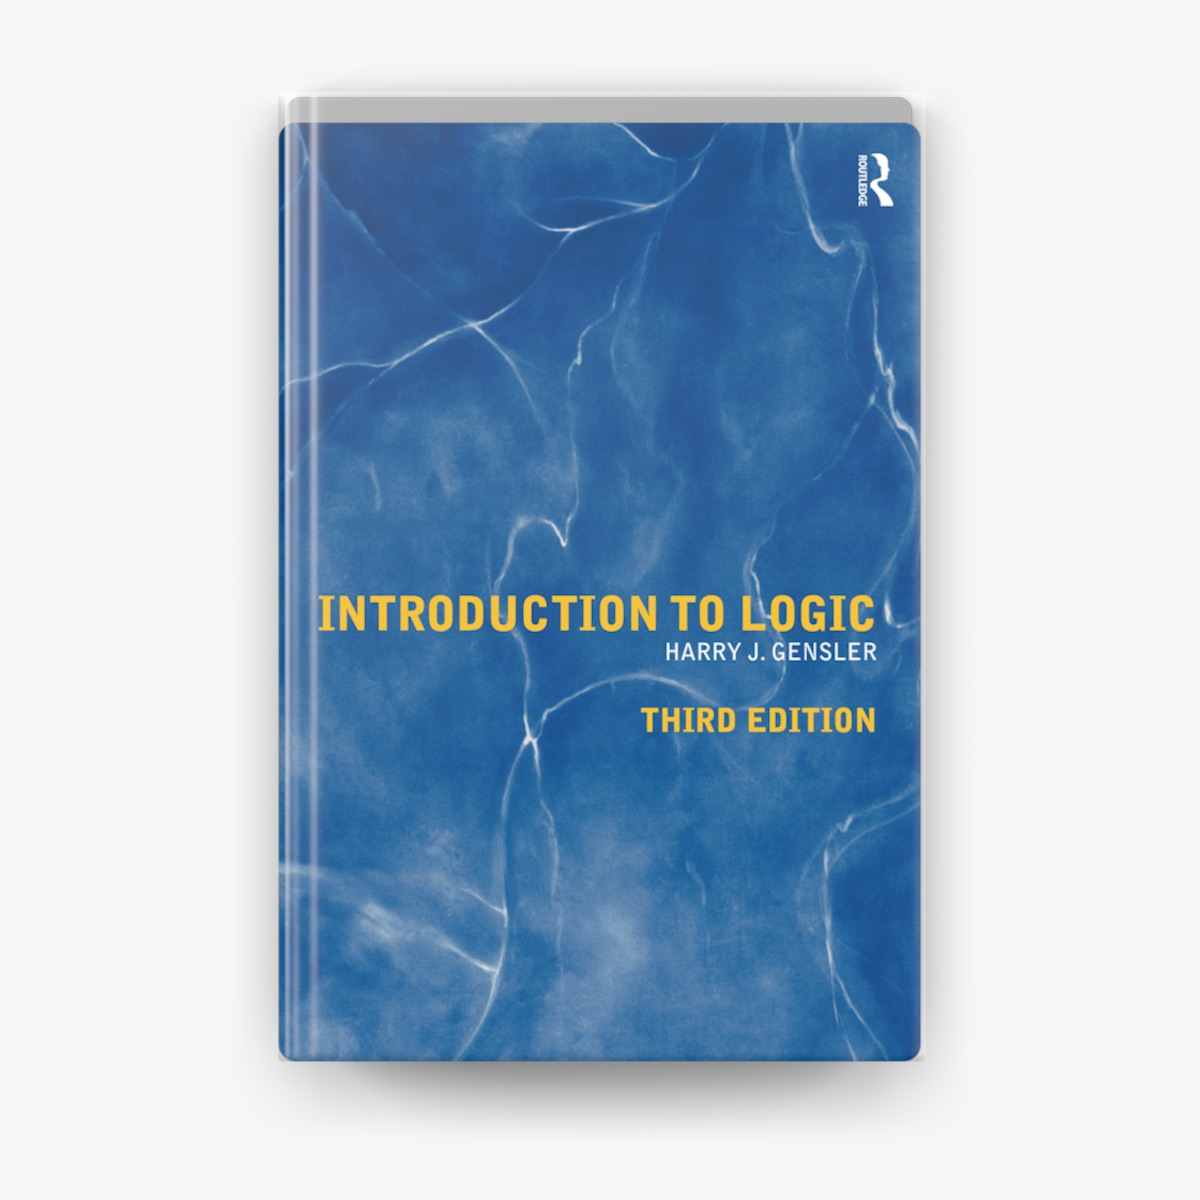
\includegraphics[height=1.9in,keepaspectratio]{assets/introduction-to-logic-cover.jpg}\par
  \smallskip
  \small\emph{Introduction to Logic}\par
  Harry J. Gensler \citep{gensler2017introduction}
\end{minipage}
\hfill
\begin{minipage}[t]{.46\textwidth}
  \centering
  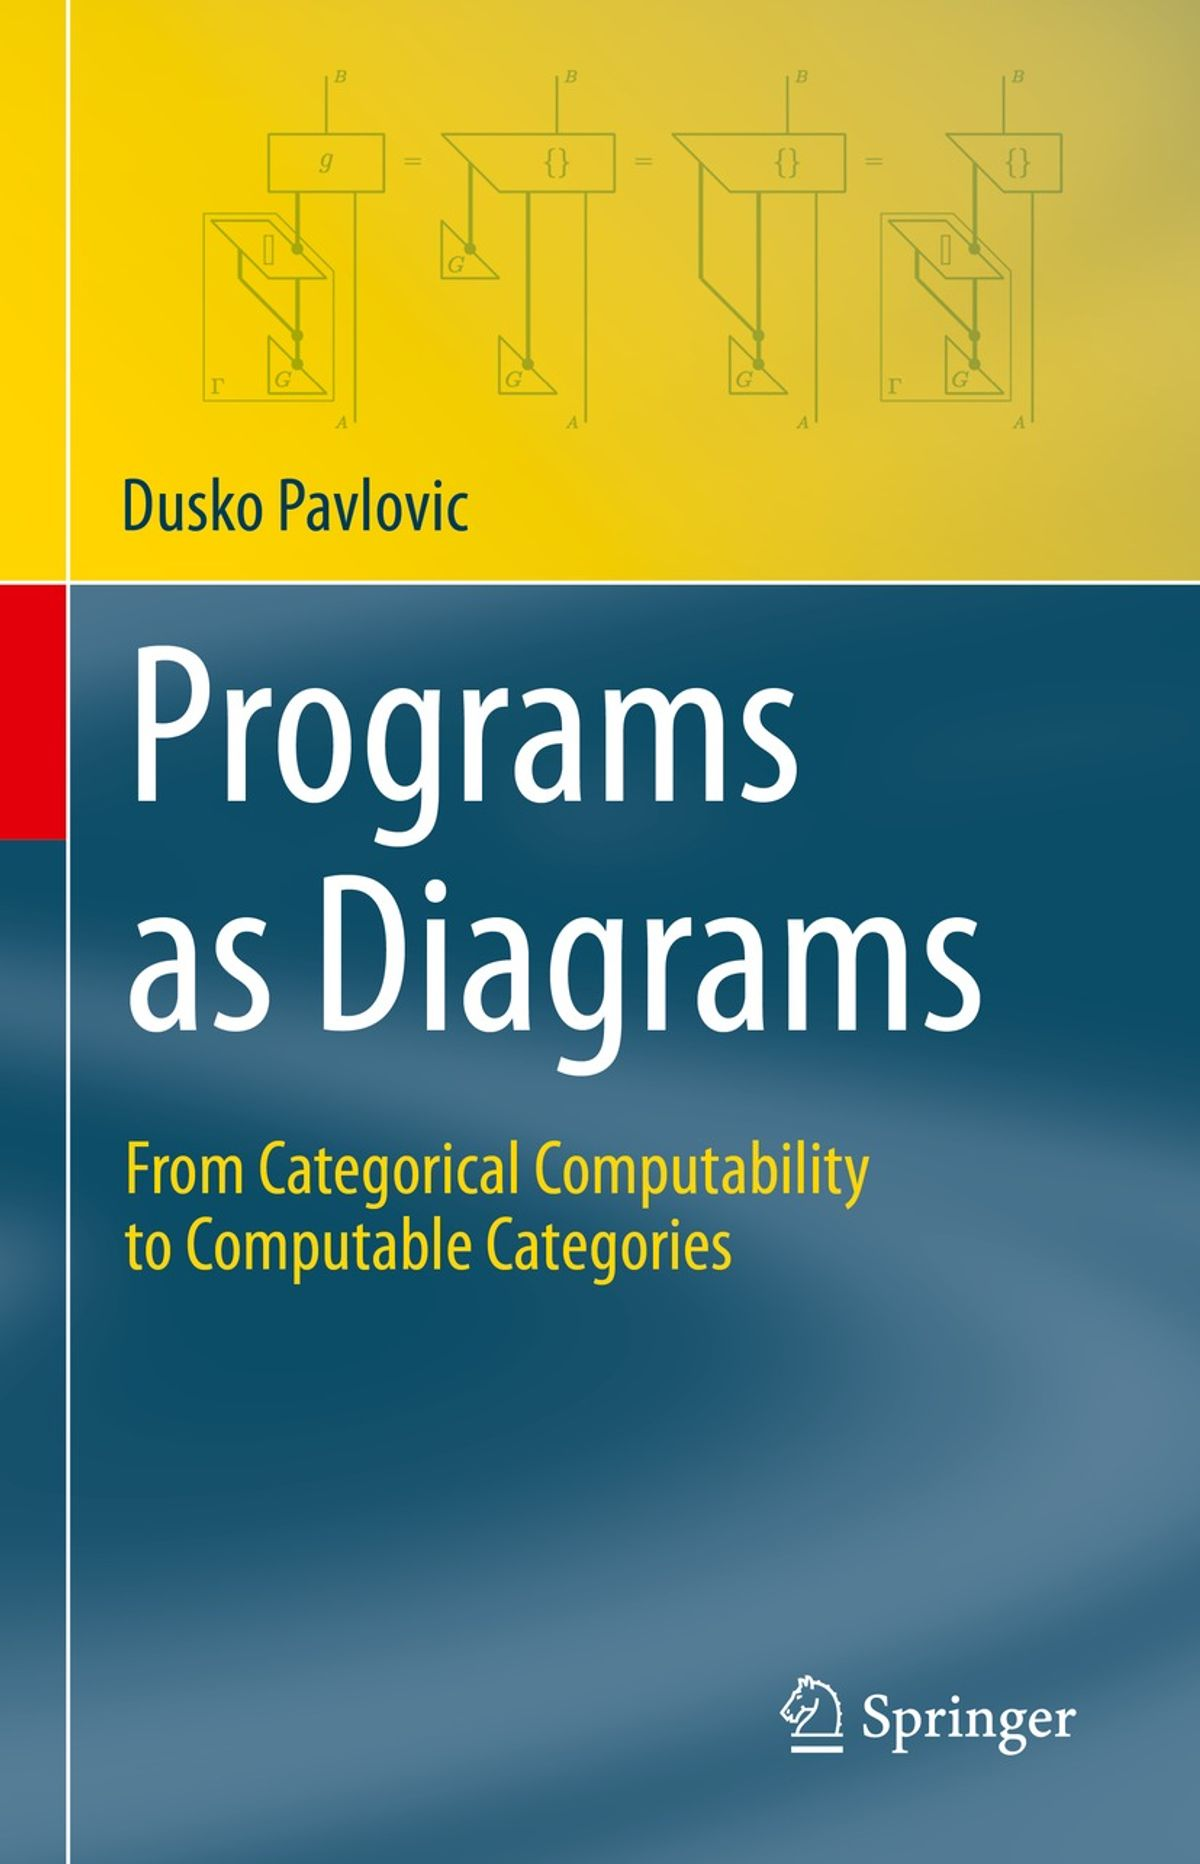
\includegraphics[height=1.9in,keepaspectratio]{assets/programs-as-diagrams-cover.jpg}\par
  \smallskip
  \small\emph{Programs as Diagrams}\par
  Dusko Pavlovic \citep{pavlovic2023programs}
\end{minipage}
\end{center}

\vspace{.55cm}

\begin{center}
\begin{minipage}[t]{.46\textwidth}
  \centering
  
\includegraphics[height=1.9in,keepaspectratio]{assets/temporal-logic-state-systems-cover.jpg}\par
  \smallskip
  \small\emph{Temporal Logic and State Systems}\par
  Fred Kr{"o}ger and Stephan Merz \citep{kroger2008temporal}
\end{minipage}
\end{center}

\vfill
{\footnotesize Cover-image sources, accessed September 25, 2026:
World Scientific edition via Kobo for Richards and Hamburger;
Open Library for Ryan et al.; Apple Books for Gensler; and Kobo's Springer
edition for Pavlovic. The Kr{"o}ger and Merz cover snapshot is from Open Library.
Cover artwork remains the property of its respective publisher.}
